%! alt Convex quadrilateral ABCD with AB = 2, BC = 9, CD = 6 and DA = 7. The diagonal AC is highlighted, and right angles are marked at B and D, so AC is the hypotenuse of both triangles ABC and ACD.
%! after_paragraph 2
%! scale 5/6
% The shared preamble of every Cevian figure. pipeline/figures turns these colours into theme-aware paint,
% and refuses any other colour, so draw only with them:
%   figink (lines and labels), figaux (construction lines), figaccent (the object the argument turns on),
%   figtint and figaccenttint (light fills).
\documentclass[border=1.5pt]{standalone}
\usepackage{tkz-euclide}
\definecolor{figink}{RGB}{0,0,0}
\definecolor{figaux}{RGB}{85,85,85}
\definecolor{figaccent}{RGB}{192,57,43}
\definecolor{figtint}{RGB}{221,221,221}
\definecolor{figaccenttint}{RGB}{245,213,208}
% tkz-euclide's defaults draw circles, compasses and marks in 50% grey and fill points with a tint.
\makeatletter
\def\tkz@otherlinecolor{figink}
\def\tkz@euc@circlecolor{figink}
\def\tkz@euc@compasscolor{figink}
\def\tkz@euc@mkcolor{figink}
\def\tkz@mk@fill{figink}
\def\tkz@euc@pointfillcolor{figink}
\makeatother
\tkzSetUpLine[color=figink,line width=.7pt]
\tkzSetUpArc[color=figink,line width=.7pt]
\tkzSetUpCompass[color=figink,line width=.5pt]
\tkzSetUpPoint[color=figink,fill=figink,size=3.1pt]
\tikzset{
  every picture/.style={line cap=round,line join=round,color=figink},
  circle style/.append style={color=figink,line width=.7pt},
  aux/.style={color=figaux,line width=.45pt,dash pattern=on 2.6pt off 2pt},
  key/.style={color=figaccent,line width=1pt},
  mk/.style={color=figink,line width=.5pt},
  lbl/.style={color=figink,inner sep=2.2pt},
  len/.style={color=figink,inner sep=1.5pt,font=\small},
}

\begin{document}
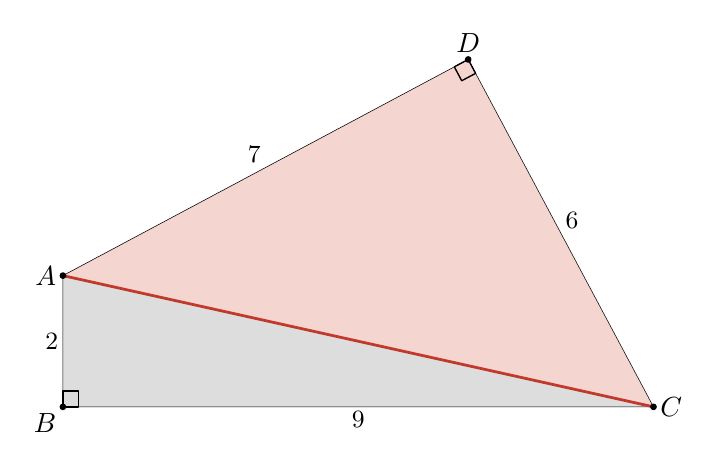
\begin{tikzpicture}
\tkzDefPoint(0.0,1.6666667){A} %! A = (0, 2)
\tkzDefPoint(0.0,0.0){B} %! B = (0, 0)
\tkzDefPoint(7.5000000,0.0){C} %! C = (9, 0)
\tkzDefPoint(5.1470588,4.4117647){D} %! D = (105/17, 90/17)
%! fact dist(A, B) == 2
%! fact dist(B, C) == 9
%! fact dist(C, D) == 6
%! fact dist(D, A) == 7
%! fact area(A, B, C, D) == 30
%! fact perp(A, B, B, C)
%! fact perp(C, D, D, A)
%! fact dist(A, C)**2 == 85
\tkzFillPolygon[color=figtint](A,B,C)
\tkzFillPolygon[color=figaccenttint](A,C,D)
\tkzDrawPolygon(A,B,C,D)
\tkzDrawSegment[key](A,C)
\tkzMarkRightAngle[size=.2,mk](A,B,C)
\tkzMarkRightAngle[size=.2,mk](C,D,A)
\tkzDrawPoints(A,B,C,D)
\tkzLabelPoint[left,lbl](A){$A$}
\tkzLabelPoint[below left,lbl](B){$B$}
\tkzLabelPoint[right,lbl](C){$C$}
\tkzLabelPoint[above,lbl](D){$D$}
\tkzLabelSegment[left,pos=.5,len](A,B){$2$}
\tkzLabelSegment[below,pos=.5,len](B,C){$9$}
\tkzLabelSegment[above right,pos=.5,len](C,D){$6$}
\tkzLabelSegment[above left,pos=.5,len](D,A){$7$}
\end{tikzpicture}
\end{document}
